\documentclass[12pt]{article}
\usepackage{graphicx}
\usepackage{setspace}
\usepackage{amsmath}
\usepackage{amssymb}
\usepackage{amsthm}
\usepackage{epstopdf}
\usepackage{tikz}
\usepackage{float}
\usepackage[ruled,vlined,boxed]{algorithm2e}
\SetKwProg{Fn}{Function}{}{}
 \usepackage{booktabs}
 \usepackage{amsmath}
\usetikzlibrary{arrows,decorations.pathmorphing,backgrounds,positioning,fit,matrix}
\RestyleAlgo{ruled}
\usepackage{url}
\topmargin -1.5cm        % read Lamport p.163
\oddsidemargin -0.04cm   % read Lamport p.163
\evensidemargin -0.04cm  % same as oddsidemargin but for left-hand pages
\textwidth 16.59cm
\textheight 21.94cm 
\parskip 7.2pt      
\LARGE
\title{\textbf{Software Component Identification and Composition}}
\vspace{2 cm}
\author{\textbf{A Colloquium Report}\\
\\
Submitted in Partial Fulfillment of Requirements for the Degree of\\
\\
Masters of Technology\\
\\\\
By\\
\textbf{Anshuman Sekhar Dash}\\
\textbf{M.Tech $3^{rd}$ Sem }\\
\textbf{Information Security}\\
\textbf{Reg. No: 2020IS04}}

\date{}
\begin{document}
\maketitle
\vspace{2 cm}
\begin{center}

\includegraphics[width=3cm,height=4cm]{logo.jpg}\\[0.1in]
\Large
\vspace{.3 cm}
\textbf{Department of Computer Science and Engineering},\\
\textbf{Motilal Nehru National Institute of Technology Allahabad, Prayagraj}.
\end{center}
\thispagestyle{empty}
\pagebreak
%\pagenumbering{Roman}
%-----------------------Undertaking --------------------------------------
%\newpage



\newpage%
\renewcommand{\baselinestretch}{1.3}
\vspace*{\fill}
\centerline{\LARGE\bf UNDERTAKING}
\vspace{3cm}
\begin{center}
	\begin{minipage}{4.5in}
		\parindent=0pt
		This is to certify, that this colloquium report submitted by me is an outcome of my independent and original work. I have duly acknowledged all the sources from which the ideas and extracts have been taken. The report is free from any plagiarism and has not been submitted elsewhere for publication.\par
		\vspace*{2cm}
		25 October, 2021\\Allahabad\par
		\hbox to 4.5in {
			\hfill\vbox{\hsize 2in\vrule width 2in height0.4pt\vspace*{-4mm}\par\center{(Anshuman Sekhar Dash)\\(Reg. no.-2020IS04)}}}
		
		\vspace*{5cm}
	\end{minipage}
\end{center}




\pagebreak
\begin{center}
	\title{	\LARGE\bf{Abstract}}
\end{center}

\normalsize

Reusing of software is found to have escalate the software engineers work output and also the craftsmanship of the final software product.
Component based software engineering (CBSE) is a unique area in software engineering wherein software components i.e a chunk of software that contains a set of related functions and data are searched for and pieced together to form a software system.This method promotes re usability and efficiency in development of software systems. CBSE's purpose is to compose software applications using plug and play software components on the framework.There are several strategies for software component identification in a system among which most widely used is object oriented based clustering.we will look into various approaches used in identifying a software component.We propose a approach which is based on clustering and formal methods to solve the problem of software component identification from a software system.The approach is based on describing a software component using formal methods and then using clustering algorithms that will groups the components in an hierarchy.when components are arranged in an hierarchical manners it provides a means to store ,browse and retrieve reusable software components.we will use the software components identified to compose a different system for comparison and demonstration of correctness of our approach used.\\[3cm]



\pagebreak
\pagenumbering{arabic}
\tableofcontents
\pagebreak
\listoffigures
\pagebreak
\listoftables
\pagebreak

\section{Motivation}
Throughout last 10 years wide spread use of software systems in many aspects of life and economy has placed new demands on the software industry for faster development of and software and also to revamp the quality of software and optimizing time take in  developing of software.One method of achieving this is to promote software reusability software reusability means reusing of software previously developed which fulfills or nearly fullfills the software requirement As is the case with many software system , no two software systems are developed the same way.Every software system differs in one or more requirements and hence software reusability will be limited unless a software system can be divided into software components each of which can be independently used in software development This is the reason for looking more into component based software engineering ,various techniques used to identify software components in a system and then composition of software systems using components.
\section{Introduction}
\subsection{What is Component Based Software Engineering}
From the last 10 years use of computer software has entered into every part of economy which has in turn generated new demand from the software industry to develop reliable and cost effective software quickly and efficiently.
Modern software systems are becoming more and more large scale which further increases the development cost , decreases the productivity and increases the cost of maintenance.
In the 90's a understanding was developed among software engineers that a software system need not be developed all the way from scratch and instead the software system can be developed by piecing together small pieces of software from previously developed software system and assembling them to make a final product.This idea was further developed into a field in software engineering named component based software engineering(CBSE).

In the context of CBSE a component will be defined as A software component is a unit of composition
with contractually specified interfaces and explicit context
dependencies only. A software component can be deployed
independently and is subject to composition by third
parties.

\begin{figure}
	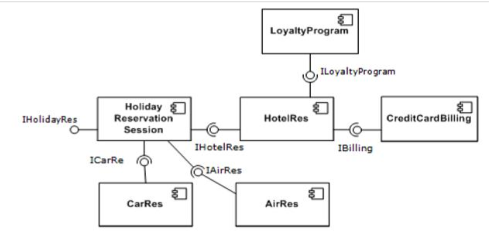
\includegraphics{softwareComponentExample.png}
	\caption{Software Components Example}
\end{figure}

In the work of \cite{componentDef} a component is defined as abstract, self-contained
packages of functionality performing a specific business function within a technology framework

This definition ascertains the fact that a software component is a well defined and independent software that gives it services using well defined interfaces.

Component-based software development is very well known and widely used as a methodology, which helps greatly in the re usability of software and reduces the cost of development significantly.

The primary role of CBSE is to direct making of software system as stitching of parts or components , development of the individual components as reusable entities and maintenance of the system developed with timely replacement of components.

Two main and important problems in Component based software development is identifying software components that can be reused and selecting of components for the development of a software system.Software component identification is one of the primary research problems in CBSE. 




\subsection{Stakeholders in Component based software Development}
\begin{itemize}
	\item \textbf{Component Developers}:-These are engineers that can be small freelance developers or an entire organisation whose job is to develop and catalogue the software components such that any further system can be developed using the software components they develop
	\item \textbf{Application Assemblers}:-Application Assemblers locate appropriate software components and according to software requirement assemble them into an integrated system.
	\item \textbf{System Developers}:-Developers are responsible for creating the software systems.They take decisions on which components to use based on the business domain and system requirements and availability of the components.They have to make a conscious decision whether to develop the requirement form scratch or use an existing software component which may be having more generalised functions. 
	\item \textbf{Customers}:-They use the systems that are developed using component based software development. Their interest lies on faster delivery of system, cheap and reliable to use.
	\begin{center}
		\begin{figure}
			\caption{Stakeholders in Component based software development}
			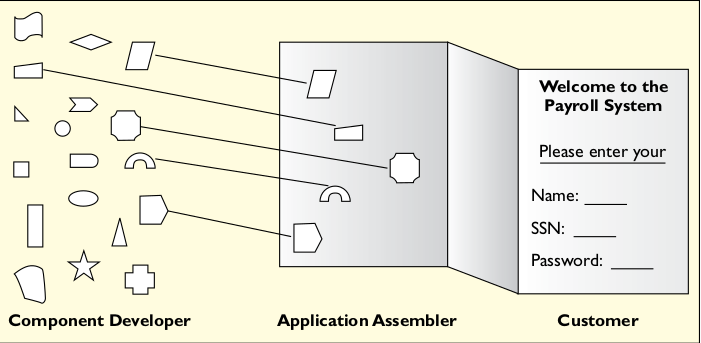
\includegraphics[scale=0.6]{stakeholders.png}
		\end{figure}
	\end{center}
	
\end{itemize}

	\begin{table}
		\caption{Artefacts used }
	\begin{center}
	\begin{tabular}{||c c ||} 
		\hline
		Artefact & References  \\ [0.5ex] 
		\hline\hline
		Static/dynamic Call graphs & \cite{graphPartion}  \\ 
		\hline
		Use Cases & \cite{neural}\cite{genetic}\cite{CRUD} \\
		\hline
		Source Code  & \cite{graphPartion} \\
		\hline
		Sequence Diagram & \cite{CRUD}\cite{2}  \\
		\hline
		Relationship between classes & \cite{genetic}  \\ [1ex] 
		\hline
		Business Model Documents & \cite{graphPartion}\cite{FCA}  \\ [1ex]
		\hline
		Class Diagrams & \cite{genetic}\cite{CRUD}  \\ [1ex]
		\hline
		Requirements Definition & \cite{highCohesionLowCoupling}  \\ [1ex]
		\hline
		Collaboration Diagram & \cite{FCA}  \\ [1ex]
		\hline
	\end{tabular}
\end{center}
\end{table}


Next there are many different methods that are used to identify components.
\subsection{Component Identification Problem}
Component identification during the software design phase is a process in which the functionalities of a given system are partitioned into non intersecting logical components to provide the starting point for designing software architecture.\cite{2}

Software component identification can be performed in two ways top-down and bottom up.
In top-down software component identification is done by analysing business domain models.
In bottom-up software component identification is done by forming reusable software components from existing software system.
One advantage of bottom up manner is that it can used with legacy systems too to identify and catalogue the software components such that it can be reused.

Identifying components from a software system is a complex problem which depends on different parameters with variable values and limiting conditions.Searching for and managing a component is difficult because a component is a run type entity.
This component identification problem belongs to Non-polynomial time problem which can only be solved by exhaustive search of all the different possibilities.

There are many techniques developed in recent years to identify components.These techniques varies according to how the components are grouped ,on what basis are the similarity of two components done\cite{9497978}.

In most of the methods the number of components needs to be known in advance but in evolutionary algorithms it is not the case.

In clustering based methods the clustering criteria includes sum of squared errors,variance ratio criterion.Some criteria also include manual weighting of features which are highly influenced by expert opinion.

The various Component identification algorithms that are studied are mentioned in table 2
\begin{table}
	\caption{Component Identification Techniques}
	\begin{center}
		\begin{tabular}{||c c ||} 
			\hline
			Methods & References  \\ [0.5ex] 
			\hline\hline
			\textbf{Clustering}& \\
			\hline
			High cohesion and Low coupling & \cite{highCohesionLowCoupling}  \\ 
			\hline
			Use Case & \cite{useCase} \\
			\hline
			\textbf{Formal Concept Analysis} &   \\ [1ex]
			\hline
			Fuzzy based analysis & \cite{fuzzy}  \\ [1ex]
			\hline
			\textbf{Evolutionary Based} &   \\ [1ex]
			\hline
			Artificial Neural Network  & \cite{neural} \\
			\hline
			Genetic Algorithm & \cite{genetic}  \\
			\hline
			Particle Swarm Optimization & \cite{pso}  \\ [1ex] 
			\hline
			\textbf{Other Methods} &   \\ [1ex]
			\hline
			CRUD Based & \cite{CRUD}  \\ [1ex]
			\hline
			Graph Partitioning & \cite{graphPartion}  \\ [1ex]
			\hline
		\end{tabular}
	\end{center}
\end{table}
\subsection{Component Composition Problem}
Correct and efficient reuse of software components not only depends on proper identification of software components from a system but also on the ways to merge the components. The other problem in CBSE is that of Component composition.Presently object oriented programming languages provide ad- hoc mechanisms for composing software using components. By providing a proper semantic foundation definition we will be able to cleanly integrate all the requirements of the software system into one system\cite{softwareComposition}.

Run time component composition for critical software systems also pose a challenge.Run time component composition is also known as dynamic composition\cite{dyanamicComp}.


\section{Methods used for solving Component Identification Problem}


\subsection{Clustering}
Clustering Algorithms which are used to identify software components contains mainly 3 steps.First, Determining the features and criteria and collection of data.Here data may refer to class object,use case diagrams,class diagrams,methods etc..Second, computing the similarity scores of the data objects collected.Third, using the clustering algorithms to group data objects and form a component.Clustering algorithms are unsupervised and doesn't need extra information for executing\cite{clusteringAna}.
\subsubsection{High Cohesion and Low Coupling}
\cite{highCohesionLowCoupling} used high cohesion and low coupling metric to cluster classes into logical components.Key classes were selected by an expert.Other classes were assigned any one among these classes based on level of dependency.It was very much dependent on the expert since key classes were required to be chosen
\subsubsection{Use Case}
Use case,object models and collaboration diagrams were used to identify components.Clustering was performed on functional dependencies of use cases.In \cite{KMeans}\cite{agglomerative} all the different types of clustering algorithms present were used and compared.It required weighting by an expert.

\subsection{Artificial Neural Network}
\cite{neural} used designing phase use case diagrams and components was generated using neural network that was self organized.The criterion for neural network was cohesion and coupling.

The data from use case diagram was extracted in the form of a matrix where each row represented sample data and each column the property. each cell denoted relationship  which was between dependency relationship,inclusion relationship and extension relationship.This matrix was normalized and initial number of cluster was calculates using mathematical equation.For the artificial neural network  x is a vector of n size which is fed to individual neurons, and highest amount of output giving neuron is selected by the transfer function.After that competitive phase,cooperative phase and adaptation phase proceeds which gives out the software components.

The number of neurons required initially is static and any change in use case the process needs to be repeated from starting.

\subsection{Genetic Algorithm}
Since evolutionary algorithms are better suited for optimisation problems and identifying software components is an optimisation problem evolutionary algorithms were used\cite{evolution}\cite{genetic}.


For genetic algorithms 4 elements are required to be defined.These are
\begin{itemize}
	\item genetic representation of the component
	\item Fitness function
	\item how to perform genetic operations i.e evolution of components
	\item the initial population
\end{itemize}
In genetic algorithm both the cohesion and coupling between two components is combined into a single objective function.This metric is then used to reject components whose fitness value is low.

The representation is known as chromosome.
\begin{figure}
	\caption{Representation of a Chromosome}
	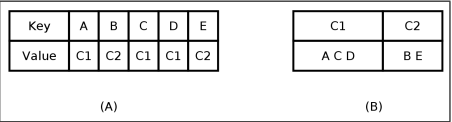
\includegraphics{chromosome.png}
\end{figure}
The chromosome consists of set of partitions of all classes. The partition is a set of non overlapping and non empty subset of all classes.
Evolutionary Algorithms are time consuming and it correctness of components depends a lot on the initial population.
Genetic algorithm generated good results in small scale systems but failed to reciprocate good results in large scale system because in large scale systems probability of getting a good initial population is very low.
\subsection{Particle Swarm Optimization}
PSO is a computational and artificial intelligence technique\cite{pso1}.The important factor of PSO which distinguishes it from other is its fast convergence in compression with other algorithms of global optimization.Feature vector is used to represent a class.
The steps performed in \cite{pso} for legacy component identification is
\begin{enumerate}
	\item Weights and Similarity measure calculation
	\item Algorithm parameters like swarm size,number of iterations , velocity equation parameters are initialized
	\item initial population generated randomly
	\item Fitness value calculation
	\item setting best particle 
	\item find the pbest and gbest
	\item interaction with software architect
	\item process repeated until desired fitness value achieved
\end{enumerate}
Shortcomings of this approach is that it can only be used with object oriented systems.
\subsection{Graph Partitioning}
In paper \cite{graphPartion} object models was related with vertices and edges of graph.
In graph partitioning technique the business model or the domain model is mapped into a weighted graph by an expert.This weighted graph is then used to apply graph segmentation technique .weights are manually assigned by experts.The graph is divided using heuristic from graph theories.

The one disadvantage of this method is that it depends a lot on the weights given by the expert.The paper didn't justify the conclusion.


\subsection{CRUD Based}

The 4 relationship used in this method is Create, Read , Write ,Update and Delete with their priority set as $C > D > U > R$ and these relationship are used to give a semantic relationship.This relationship is then transformed into a matrix .\cite{CRUD}Used business events as inputs.

\subsection{Formal concept analysis Based}
FCA is a framework which uses mathematics that is used to
explain and analyse data and their relationships\cite{FCA1}.

\cite{FCA} uses a framework based on FCA that divides class diagram into logical components which is like that of clustering techniques.Adding on this paper \cite{FCA} used a new method that was based on fuzzy FCA.Dispersion and distance concept was used to calculate cohesion and coupling metrics.Here a component may belong to more than one cluster.A degree of membership is given to every component with every cluster.a degree of 0 will mean that the respective component does not belong to this cluster.a degree of 1 will mean that the respective component only belongs to the cluster given. Fuzzy clustering  is useful when the boundaries between clusters are not well separated.


Disadvantage of this method was that the threshold for dispersion and distance was set manually and it impacted heavily on the result.It also depends on the number of clusters and is susceptible to outliers in the components data.
\section{Constructing Software Library using formal Methods}
After studying all the previous works we found many limitation that need to be taken care of.Few of the solutions used use case diagrams , class diagrams which are domain level and will be difficult to implement on legacy systems.It is only top down solution and requires prior knowledge of the overall system with the use of use case diagrams sequence diagram etc.These domain models are dependent on how the domain models were formed and is not standardised. Few solution only focused on object oriented systems which cannot be used with procedural and functions based systems.Keeping all the above limitations our solution will be based on bottom up approach and will work on already developed software systems.
We Propose a solution where individual software components will be specified using predicate logic\cite{formalFromCode}.
We selected \cite{formal} and \cite{survey} as the base paper for our proposed solution.\cite{formal} used formal language predicate logic to specify software components which can be used for both object oriented and function based systems.since it only requires the source code to specify software components no domain level elements are required from the software system.\cite{survey} mentions the metrics which will be used to calculate the corrected of our solution.
The specification of a software component will contain an abstract data type and the set of methods that operates on the abstract data type.
each of this method will contain interface, type declarations , a precondition and a post condition.
\begin{figure}
	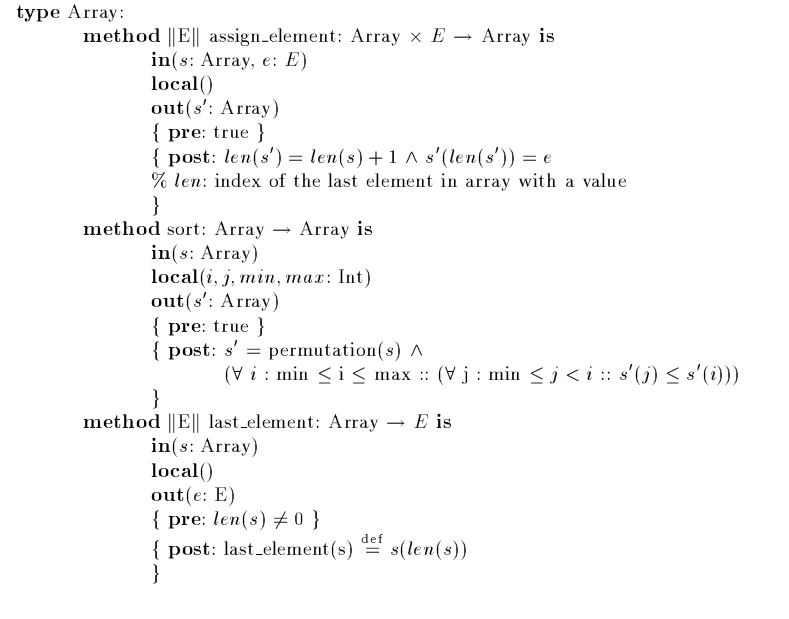
\includegraphics[scale=0.5]{example_formal.png}
	\caption{Example of predicate logic specification of component}
	\cite{formal}
\end{figure}
The steps are as follows:-
\subsection{Formal Specification of Software components}
Interface represents syntactic specification of the method.
type declarations represents the the type of input output and local variables used.
precondition describes the condition of the variables before the method is called
post condition describes the condition of the variables after the method is called.
The specification follows all the predicate logic conventions such as conjunction dis-junction,rules of inference etc.

\subsection{Lower level hierarchy}
We will first generate the lower level hierarchy using the formal specification of software components.
The lower level hierarchy will generate fine-grained components on which logical reasoning can be done on the basis of specifications.

The subsumption relationship between 2 components will be used to classify and group together components which can be reused.
A component is said to subsume another component when the first component is more general than the second.
This abstract data type can be implemented on classes as class can also be termed as an abstract data type.


The lower level hierarchy will be generated by comparing components formed  using pair wise comparison algorithm.
\begin{algorithm}
	\caption{Pair Wise Algorithm}
	\KwIn{The set of components from subsumption test algorithm $S=\{Cmp_1,Cmp_2,...,Cmp_n\}$}
	\KwOut{Hierarchy of components by applying generality principle}
	\While{$S\neq\{\}$}
	{
		choose some $Cmp_i \mathcal{E}  S $;\\
		$S \leftarrow S\div Cmp_i$;\\
		$set \leftarrow S$;\\
		\While{$set \neq \{\}$}
		{
			choose some $Cmp_j \mathcal{E}  S $;\\
			$S \leftarrow S\div Cmp_j$;\\
			\If{$C_i \sqsupseteq C_j$}
			{$C_i$ is set as parent of $C_j$ }
			\ElseIf
			{$C_j \sqsupseteq C_i$}
			{$C_j$ is set as parent of $C_i$}
		}
		
	}
\end{algorithm}
\begin{figure}
	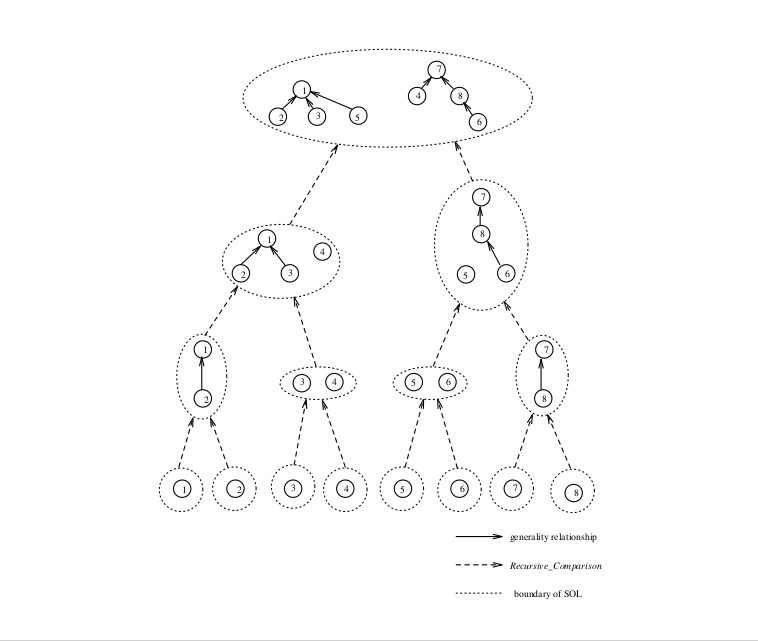
\includegraphics[scale=0.6]{lowerLevelHierarchy.png}
	\caption{Lower Level Hierarchy Building using recursive comparison\cite{formal}}
	
\end{figure}

After generating the lower hierarchy of software components in order to form a connect hierarchy clustering algorithm will be done.

The objective to clustering algorithm is to create a set of clusters with low inter cluster similarity and high intra cluster similarity.
\subsection{Measuring Similarity}
Similarity of 2 components is represented as \(S(x,y)\).
In our solution a component is represented in disjunctive normal form consisting of conjuncts. Each conjunct is to be associated with an equivalence class.Example \(X=(C_1 \wedge C_2)\vee(C_2 \wedge C_3)\ and \ Y=(C_3)\vee(C_2 \wedge C_3)\).For our solution we will use equivalence class as greater(a,b).
using all the above information for every component a matrix will be constructed whose dimensions are \(m \times (T+1)\) where m is the number of conjunction and T is the number of equivalence classes.

the matrix will be filled according to the formula below.
here x(i,j) represents entry in row i and column j.
row i denotes the $i^{th}$ disjunction of the component x .
\begin{center}
	\(X(i,0) = u_i\;  0 \leqq i \leqq m \leqq 1\;and 
	X(i,j) = l\;  x_i\;has\;l\;terms\;in\;eq\;class\;j
	\)
\end{center}

Similarly \(Y\) matrix was filled.


from the above 2 matrices that were derived the similarity matrix will be constructed 
\begin{center}
	\(
	for\ all\ i,j\ if\ X(i,0)=Y(j,0)
	)\
	\)
	\\
	\(
	then\ s^{'} (i,j)=\frac{\sum_{t=1}^{T}2*min(X(i,t),Y(j,t))}{(X(i,t)+Y(j,t)}\)
	\\
	\(else\ s^{'}(i,j)=0
	\)
\end{center}

Using all the above formulas the similarity between two components is given as 
\begin{center}
	\(s(X,Y)\)=$\frac{\sum_{i=1}^{m}\sum_{j=1}^{n}s^{'}(i,j)}{N}$
\end{center}


\subsection{Higher Level Hierarchy using Clustering Algorithm}
Cluster analysis or clustering is the project of grouping a set of items in the sort of manner that objects in the same group (called a cluster) are more comparable (in some experience) to every aside from to the ones in different group (clusters). It is a main task of exploratory information analysis, and a common technique for statistical data analysis, used in many fields, along with sample recognition, photo analysis, statistics retrieval, bioinformatics, information compression, computer photographs and machine learning. Cluster analysis on its own isn’t always one unique algorithm, but the preferred task to be solved. It may be completed by way of diverse algorithms that range extensively in their know-how of what constitutes a cluster and how to efficaciously find them. Popular notions of clusters consist of businesses with small distances between cluster individuals, dense areas of the facts space, periods or precise statistical distributions. Clustering can therefore be defined as a optimisation problem with multiple objectives. The appropriate clustering set of rules and parameter settings (such as parameters which includes the distance characteristic to apply, a density threshold or the variety of anticipated clusters) depend upon the person information set and supposed use of the results. Cluster analysis as such isn’t always an automatic mission, but an iterative system of information discovery or interactive multi-objective optimisation that entails trial and failure. It is frequently essential to alter information preprocessing and model parameters till the end result achieves the preferred houses. There isn’t any objectively accurate clustering set of rules, however as it became referred to, clustering choice and parameters lies with that of the programmer. The maximum suitable clustering algorithm for a particular problem often desires to be chosen experimentally, except there’s a mathematical purpose to prefer one cluster version over another. An algorithm that is designed for one form of version will generally fail on a information set that carries a greatly exclusive type of model. For example, k-method can’t discover non-convex clusters. Clustering algorithms can be separated into 2 categories.One is divisive algorithms and the other is agglomerative algorithms. For divisive algorithms the set X is further divided into a group of clusters using measure of dissimilarity which creates a finer partition. While in agglomerative algorithms a group of finer partitions are merged together using similarity measures to form a courser partition.Each intermediate steps helps in generating a hierarchy of clusters.It gives an understanding of the architecture of the system.The similarity measure is an important factor in the agglomerative hierarchical clustering algorithms. The agglomerative hierarchical clustering algorithms (AHCA) begin from a set of individual entities that are first allocated into small clusters which are then in turn allocated into larger clusters until reaching a final all inclusive clustering. We will be using Agglomerative Clustering since we are identifying components from a software system that is bottom up approach.

\begin{figure}
	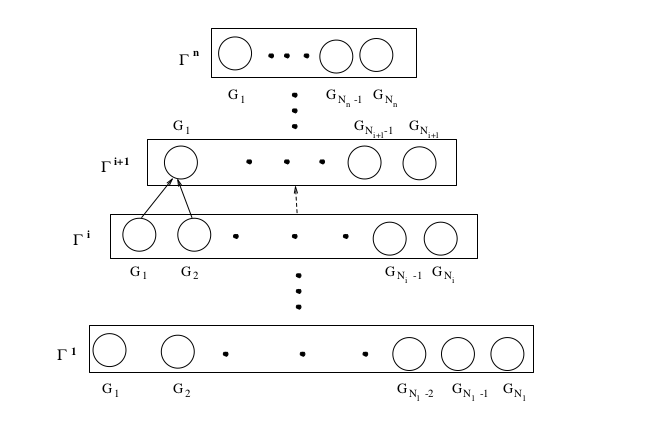
\includegraphics[scale=0.7]{agglomerativeClustering.png}
	\caption{Visual representation of Agglomerative Clustering\cite{formal}}
	
\end{figure}

\begin{algorithm}
	\caption{Agglomerative Clustering}\label{alg:cap}
	\KwIn{A Set of disjoint Lattices}
	\KwOut{Set of Clusters Unified into one}
	\begin{enumerate}
		\item each top element of the lattice is set a cluster with only single element
		\item search for a pair of clusters which have maximum similarity 
		\item merge the the top 2 most similar clusters into a new cluster
		\item calculate new similarity scores for the clusters left
		\item proceed until only one cluster is left
	\end{enumerate}
\end{algorithm}
\section{Conclusion \& Recommendation for Future Researches}
\subsection{Conclusion}
We looked into what is component based software engineering,its main problem.We further discussed on various types of approaches taken for component identification problem in component based software development.We determined that Clustering based technique is most extensively used but the approaches here were limited to domain based models and not the actual source code.A different method was needed to use describe a component and which is why use of predicate logic was proposed.Specifying software components using predicate logic will help in also describing legacy systems.We divided our technique to lower level hierarchy and higher level hierarchy.The lower level hierarchy generates the fine grained components which will be used in software reusing.In higher level hierarchy for easy searching and generating a hierarchy of software components clustering will be used.For clustering method we proposed a similarity measuring formula based on absolute weighting scheme.After getting the similarity measure and the lattice for the input to clustering algorithm we used agglomerative clustering since we desired for a bottom up approach.In higher level hierarchy clustering to generate a hierarchy of software components for smooth and fast searching clustering will be used.For clustering method we proposed a similarity measuring formula based on absolute weighting scheme.After getting the similarity measure and the lattice for the input to clustering algorithm we used agglomerative clustering since we desired for a bottom up approach.

\begin{figure}[H]
	
	\begin{center}
		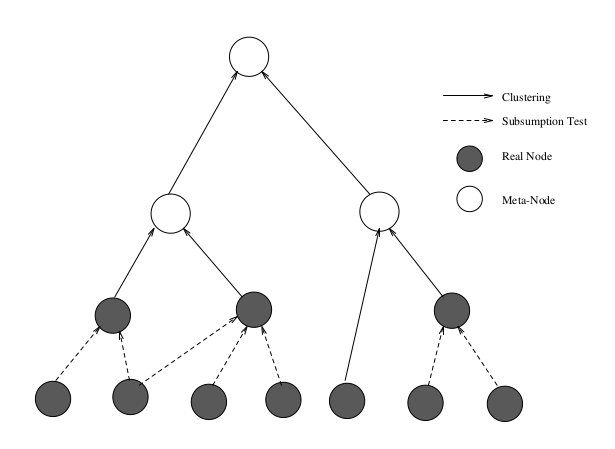
\includegraphics[scale=0.4]{finalHierarchy.png}
	\end{center}
	\caption{Final resultant hierarchy of software components\cite{formal}}
	

\end{figure}
\subsection{Recommendation for future research}
In future research we plan to use the proposed solution on various software systems which will generate reusable components.A variety of software systems will be taken such as Parking Lot system,Chain store system,Library Management system,Online marks analysis system,A B2B auction system for which components will be identified using our proposed solution.These components will be catalogued.Further we will look into composition problem of CBSE and try to find a solution to compose a Airport System using the components catalogue and composition solution.  We will use these reusable components to develop our own software system and calculate various metrics like lines of code, number of reusable components degree of coupling and cohesion etc.
\\Tools we will be using for building the solution:-
\begin{enumerate}
	\item AUTOSPEC tool to extract formal specifications from primary programming structures of the source code
	\item Jupyter notebook for writing and running of python code for clustering 
\end{enumerate}

We will also look into using evolutionary methods with formal methods since evolutionary methods gives a good result in optimization problems.In a quick look, the particle swarm optimization and artificial neural network methods looked promising and using formal methods along with them guarantees to give out better results.

\bibliographystyle{plain}
\bibliography{ref}
\end{document}
